\chapter{Zestawienie zbiorcze i podsumowanie}

\section{Oferowane funkcjonalności}

Omówione w ramach niniejszej pracy biblioteki różnią się typem i liczbą oferowanych funkcjonalności. Tabela \ref{fun:sum} zbiorczo podsumowuje poszczególne omówione w poprzednich rozdziałach aspekty.

\begin{longtable}{c | c | c | c}
	\centering
	\multirow{2}{*}{\makecell{Funkcjonalność}} & \multicolumn{3}{c}{Biblioteka} \\
	\cline{2-4}
	 &  Shogun & Shark-ML & Dlib \\
	\hline
	\makecell{Odczyt \\ danych} & \makecell{std::vector, \\ wsparcie dla \\ formatu CSV} & \makecell{surowe \\ tablice, \\ wsparcie dla \\ formatu CSV, \\ wsparcie \\ dla HTTP} & \makecell{std::vector, \\ wsparcie dla \\ formatu CSV} \\
	\hline
	{Normalizacja} & min-max & \makecell{przedział \\ jednostkowy, \\ jednostkowa \\ wariancja, \\ zerowa \\ średnia i \\ wybrana \\ wariancja} & standaryzacja \\
	\hline
	\makecell{Redukcja \\ wymiarowości} & \makecell{PCA, Kernel PCA, \\ MDS, IsoMap, \\ ICA, Factor analysis, \\t-SNE} & \makecell{PCA, Liniowa \\ analiza \\ dyskryminacyjna} & \makecell{PCA, Liniowa \\ analiza \\ dyskryminacyjna, \\ Mapowanie \\ Sammona} \\
	\hline
	\makecell{Regularyzacja} & \makecell{L1 i L2 \\ automatyczna} & \makecell{L1 i L2} & L2 \\
	\hline
	\makecell{Regresja \\ liniowa} & Tak & Tak & Tak \\
	\hline
	\makecell{Regresja \\ logistyczna} & Tak & Tak & Nie \\
	\hline
	\makecell{Maszyna \\ wektorów \\ nośnych} & Tak & Tak & Tak \\
	\hline
	\makecell{Algorytm \\ K-najbliższych \\ sąsiadów} & Tak & Tak & Nie \\
	\hline
	\makecell{Algorytm \\ zbiorowy} & \makecell{Wzmacnianie \\ gradientu, \\ losowy las} & \makecell{Losowy \\ las} & Nie \\
	\hline
	\makecell{Sieć \\ neuronowa} & Tak & Tak & Tak \\
	\hline
	\makecell{Jądrowa \\ regresja \\ grzbietowa} & Nie & Nie & Tak \\
	\hline
	\makecell{Błąd \\ średniokwadratowy} & Tak & Tak & Nie \\
	\hline
	\makecell{Średni \\ błąd \\ bezwzględny} & Tak & Tak & Nie \\
	\hline
	\makecell{Błąd typu \\ zero-jeden} & Nie & Tak & Nie \\
	\hline
	\makecell{Błąd \\ dyskretny} & Nie & Tak & Nie \\
	\hline
	\makecell{Entropia \\ krzyżowa} & Nie & Tak & Nie \\
	\hline
	\makecell{Kawałkami \\ liniowa \\ funkcja straty} & Nie & Tak & Nie \\
	\hline
	\makecell{Średnio-\\kwadratowy \\ błąd typu \\ kawałkami \\ liniowej \\ funkcji straty} & Nie & Tak & Nie\\
	\hline
	\makecell{Kawałkami \\ liniowa \\ funkcja straty \\ typu epsilon} & Nie & Tak & Nie\\
	\hline
	\makecell{Średnio-\\kwadratowy \\ błąd kawałkami \\ liniowej funkcji \\ straty typu \\ epsilon} & Nie & Tak & Nie\\
	\hline
	\makecell{Funkcja \\ straty \\ Hubera} & Nie & Tak & Nie\\
	\hline
	\makecell{Funkcja \\ straty \\ Tukeya} & Nie & Tak & Nie\\
	\hline
	\makecell{Logarytmiczna \\ funkcja \\ straty} & Tak & Nie & Nie\\
	\hline
	\makecell{Metryka $R^2$} & Tak & Tak & Nie\\
	\hline
	\makecell{Dokładność} & Tak & Nie & Tak \\
	\hline
	\makecell{Pole pod \\ wykresem \\ ROC} & Tak & Tak & Tak* \\
	\hline
	\makecell{Sprawdzian \\ krzyżowy \\ k-krotny} & Tak & Tak & Tak \\
	\caption{Zbiorcze porównanie funkcjonalności bibliotek.}
	\label{fun:sum}
\end{longtable} 

* - konieczność przeliczenia pola na podstawie uzyskanych punktów pomiarowych wykresu funkcji.

Analizując dane zebrane w tabeli \ref{fun:sum} można zauważyć, że biblioteki Shogun oraz Shark-ML są bardzo zbliżone do siebie typem i liczbą dostępnych metod uczenia maszynowego, jednak Shark-ML posiada więcej rodzajów błędów możliwych do wykorzystania jako funkcje strat, pozwalając na większą swobodę względem dostosowywania procesu uczenia. Najmniejszą liczbą funkcjonalności charakteryzuje się biblioteka Dlib, posiadająca jedynie podzbiór algorytmów dostępnych w innych projektach. Ponadto, posiada ona bardzo ubogie możliwości analizy sprawności modeli, wymagając od użytkownika napisania własnych procedur przetwarzania uzyskanych danych, jak np. procedura obliczania pola pod wykresem krzywej charakterystycznej odbiornika.

\section{Porównanie wyników dla zadanych przykładów}

W celu przetestowania sprawności poszczególnych bibliotek, użyto ich do stworzenia i ewaluacji modeli regresji liniowej oraz maszyny wektorów nośnych dla zestawów danych opisanych w rozdziale 3. Dla każdego modelu użyto 80\% zestawu danych w celu treningu, oraz pozostałe 20\% jako dane testowe. Tabela \ref{tab:models} przedstawia zbiorcze zestawienie uzyskanych wyników ewaluacji. Wyjście programów zostało zaprezentowane na rysunkach \ref{fig:shogun_linear_svm}, \ref{fig:shark_linear_svm} oraz \ref{fig:dlib_linear_svm}.

\newpage
\begin{longtable}{c | c | c }
	\centering
	\multirow{2}{*}{\makecell{Biblioteka}} & \multicolumn{2}{c}{Metoda uczenia maszynowego} \\
	\cline{2-3}
	& Regresja liniowa & Maszyna wektorów nośnych \\
	\hline
	\makecell{Shogun} & \makecell{Dane treningowe: \\ MSE = 0,903031; $R^2$ = 0,407058 \\ Dane testowe: \\ MSE = 1,26897; $R^2$ = -0.127851} & \makecell{Dane treningowe: \\ AUC ROC: 1 \\ Dane testowe: \\ AUC ROC: 0,5} \\
	\hline
	\makecell{Shark} & \makecell{Dane treningowe: \\ MSE = 0,38728; $R^2$ = 0,745707 \\ Dane testowe: \\ MSE = 0,449118; $R^2$ = 0,60082} & \makecell{Dane treningowe: \\ AUC ROC: 1 \\ Dane testowe: \\ AUC ROC: 0,5} \\
	\hline
	\makecell{Dlib} & \makecell{Dane treningowe: \\ MSE = 3,08953; \\ Dane testowe: \\ MSE = 1,33014; } & \makecell{Dane treningowe: \\ AUC ROC: 1 \\ Dane testowe: \\ AUC ROC: 1} \\
	\caption{Zestawienie uzyskanych wyników poprawności modeli.}
	\label{tab:models}
\end{longtable} 

\begin{figure}[!ht]
	\centering
	\begin{minipage}{0.31\textwidth}
		\centering
		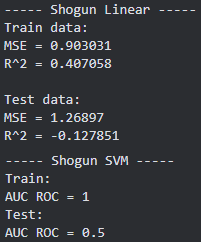
\includegraphics[width=0.8\linewidth]{Rozdzial7/shogun}
		\caption{Wynik działania programu dla biblioteki Shogun}
		\label{fig:shogun_linear_svm}		
	\end{minipage}%
    \hspace{0.02\textwidth}
	\begin{minipage}{0.31\textwidth}
		\centering
		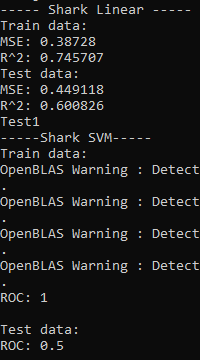
\includegraphics[width=0.7\linewidth]{Rozdzial7/shark}
		\caption{Wynik działania programu dla biblioteki Shark}
		\label{fig:shark_linear_svm}		
	\end{minipage}%
	\hspace{0.02\textwidth}
	\begin{minipage}{0.31\textwidth}
		\centering
		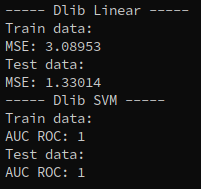
\includegraphics[width=0.8\textwidth]{Rysunki/Rozdzial7/dlib}
		\caption{Wynik działania programu dla biblioteki Dlib}
		\label{fig:dlib_linear_svm}
	\end{minipage}
\end{figure}

Analizując powyższe wyniki pod krątem regresji liniowej, stwierdzić można iż pierwsze miejsce zajęła biblioteka Shark-ML cechując się najniższymi błędami średniokwadratowymi. Na drugim miejscu znalazła się biblioteka Shogun. Zauważyć można, że mechanizm wyliczania współczynnika determinacji liniowej $R^2$ wyszedł dla danych testowych poza dopuszczalny zakres. Podejrzewa się, iż jest to wynik kumulacji błędów reprezentacji zmiennoprzecinkowej wartości podczas obliczeń, wskazując że mechanizm wyliczania składowych potrzebnych do obliczenia $R^2$ dla tej biblioteki jest niestabilny numerycznie. Ostatnie miejsce zajęła biblioteka Dlib, w przypadku której wartość błędu średniokwadratowego przekroczyła 3 jednostki.

Dużo gorsze rezultaty uzyskane zostały przy próbie dokonania klasyfikacji z wykorzystaniem wyżej wspomnianych bibliotek. Każda z nich cechuje się pozornie idealnym dopasowaniem do danych uczących, oraz w przypadku bibliotek Shark-ML i Shogun dopasowaniem porównywalnym do klasyfikacji za pomocą rzutu monetą. Biblioteka Dlib dodatkowo uzyskała pole pod wykresem krzywej charakterystycznej odbiornika na poziomie 1 dla danych testowych. Powyższe wyniki są nierealne do uzyskania, co udowodniono w rozdziale 3.3.1, wykorzystując dedykowane oprogramowanie statystyczne. W związku z tym rozpoczęto analizę przyczyny uzyskanych wyników. 

W celu poprawy uzyskanych wyników i rozwiązania napotkanych błędów zdecydowano się na normalizację wartości predyktorów dla obu zestawów danych do przedziału $[0; 1]$ z wykorzystaniem programu JMP, a następnie analizę kodu realizującego uczenie maszyn wektorów nośnych w poszczególnych bibliotekach. Pierwszą z analizowanych bibliotek była biblioteka Shark-ML, w przypadku której wykorzystano ręczne dostrajanie parametrów gamma oraz regularyzacji. Okazało się, że po normalizacji oraz ustawieniu parametrów gamma na 0,16 oraz regularyzacji na 1 uzyskano prawidłowi i prawdopodobne pole pod wykresem na poziomie 0,933129 dla danych testowych. W drugiej kolejności przetestowano bibliotekę Shogun. Niestety pomimo normalizacji danych nie udało się rozwiązać problemu ujemnego współczynnika $R^2$ dla danych testowych, natomiast poprawie udało się wykonać klasyfikację, uzyskując wartość pola pod wykresem krzywej charakterystycznej odbiornika wynoszącą 0,638112. Należy zwrócić szczególną uwagę, że normalizacja pogorszyła uzyskane wyniki przed bibliotekę Shogun, zmniejszając uzyskane $R^2$ dla danych uczących i sprawiając, że $R^2$ dla danych testowych jeszcze bardziej odbiega od swojego prawidłowego zakresu. Ostatnią z bibliotek była biblioteka Dlib, dla której normalizacja zestawu danych dla zadania regresji znacznie poprawiła uzyskany błąd średniokwadratowy, natomiast w dalszym ciągu uzyskane zostało idealne dopasowanie maszyny wektorów nośnych, co może wskazywać na to, iż nie jest on zaimplementowany prawidłowo w bibliotece. Tabela \ref{tab:models2} podsumowuje wyniki uzyskane po analizie kodu oraz normalizacji danych. Wyjście programów zostało przedstawione na rys. \ref{fig:shogun_linear_svm2}, \ref{fig:shark_linear_svm2} oraz \ref{fig:dlib_linear_svm2}

\begin{longtable}{c | c | c }
	\centering
	\multirow{2}{*}{\makecell{Biblioteka}} & \multicolumn{2}{c}{Metoda uczenia maszynowego} \\
	\cline{2-3}
	& Regresja liniowa & Maszyna wektorów nośnych \\
	\hline
	\makecell{Shogun} & \makecell{Dane treningowe: \\ MSE = 0,0286481; $R^2$ = 0,3127 \\ Dane testowe: \\ MSE = 0.0427863; $R^2$ = -0.389462} & \makecell{Dane treningowe: \\ AUC ROC: 0,789143 \\ Dane testowe: \\ AUC ROC: 0,638112} \\
	\hline
	\makecell{Shark} & \makecell{Dane treningowe: \\ MSE = 0,0105995; $R^2$ = 0,745707 \\ Dane testowe: \\ MSE = 0.0122919; $R^2$ = 0,600826} & \makecell{Dane treningowe: \\ AUC ROC: 0,921643 \\ Dane testowe: \\ AUC ROC: 0,933129} \\
	\hline
	\makecell{Dlib} & \makecell{Dane treningowe: \\ MSE = 0,481402; \\ Dane testowe: \\ MSE = 0,179538; } & \makecell{Dane treningowe: \\ AUC ROC: 1 \\ Dane testowe: \\ AUC ROC: 1} \\
	\caption{Zestawienie uzyskanych wyników poprawności modeli.}
	\label{tab:models2}
\end{longtable} 

Podsumowując, zauważono że każda z bibliotek jest wyjątkowo wrażliwa na zakres wartości predyktorów i w celu prawidłowego wykorzystania przeważnie wymaga, aby każdy z predyktorów zawierał się w przedziale $[0; 1]$. W przypadku zestawu danych klasyfikacyjnych było to szczególnie widoczne, gdyż ze względu na bardzo duże wartości zmiennych po transformacji odwrotnym wzorem Arrheniusa, istniała duża rozbieżność między ich zakresem, a zakresami pozostałych predyktorów. Ponadto zauważono, że mechanizm obliczania współczynnika determinancji liniowej w bibliotece Shogun oraz model maszyny wektorów nośnych w bibliotece Dlib najprawdopodobniej posiadają błędy implementacji, a więc należy z nich nie korzystać, lub mieć do nich bardzo ograniczony stopień zaufania. Spośród uzyskanych wyników, najlepszym dopasowaniem do danych charakteryzuje się biblioteka Shark, na drugim miejscu znalazła się biblioteka Shogun, natomiast ostatnie miejsce zajęła biblioteka Dlib.


\begin{figure}[!ht]
	\centering
	\begin{minipage}{0.31\textwidth}
		\centering
		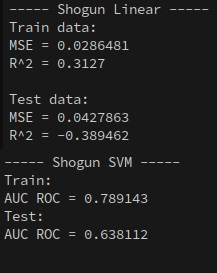
\includegraphics[width=0.8\linewidth]{Rozdzial7/shogun_linear_svm}
		\caption{Wynik działania programu dla biblioteki Shogun}
		\label{fig:shogun_linear_svm2}		
	\end{minipage}%
	\hspace{0.02\textwidth}
	\begin{minipage}{0.31\textwidth}
		\centering
		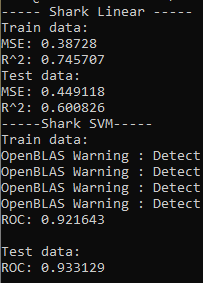
\includegraphics[width=0.7\linewidth]{Rozdzial7/shark_linear_svm}
		\caption{Wynik działania programu dla biblioteki Shark}
		\label{fig:shark_linear_svm2}		
	\end{minipage}%
	\hspace{0.02\textwidth}
	\begin{minipage}{0.31\textwidth}
		\centering
		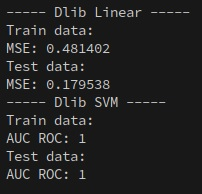
\includegraphics[width=0.8\textwidth]{Rysunki/Rozdzial7/dlib_linear_svm}
		\caption{Wynik działania programu dla biblioteki Dlib}
		\label{fig:dlib_linear_svm2}
	\end{minipage}
\end{figure} 

\section{Wymagany nakład pracy i jakość źródeł}

W procesie pracy z poszczególnymi bibliotekami zauważono, że najmniejszą ilością potrzebnego wkładu pracy charakteryzowała się biblioteka Shark-ML. Wynika to z bardzo przyjaznej dla użytkownika składni, oraz dokładnej dokumentacji dostępnej na stronie internetowej projektu, wraz z przykładami wykorzystania poszczególnych metod. Biblioteka także bez jakichkolwiek problemów została zbudowana i zainstalowana na systemie operacyjnym Ubuntu 22.04 w środowisku WSL2, pozwalając bardzo szybko przejść do badań.

Drugą biblioteką pod względem koniecznego wkładu czasu okazał się zestaw narzędziowy Dlib. Posiada on stronę projektu z wylistowanymi klasami oraz funkcjami dostępnymi w bibliotece, jednak opis działania poszczególnych metod jest bardzo pobieżny, oraz brakuje dostępnych przykładów. Składnia biblioteki może stanowić wyzwanie dla użytkownika, gdyż nie zawsze jest oczywista, i momentami utrudnia analizę realizowanych przez program operacji.

Jako najbardziej wymagającą bibliotekę uznano Shogun. W chwili pisania niniejszej pracy, zarówno oficjalne repozytorium projektu jak i repozytorium dystrybucji dla systemu operacyjnego Ubuntu okazało się być niekompletne. Uniemożliwiło to zainstalowanie biblioteki za pomocą wbudowanego managera pakietów oraz zbudowanie jej ze względu na nienaprawione zależności do przeniesionych repozytoriów stron trzecich. Mimo przyjaźniejszej składni niż w przypadku Dlib, wspomniany wcześniej mankament sprawia, że w celu pobrania biblioteki konieczne okazało się zainstalowanie specjalnego managera pakietów \textit{nix} posiadającego starszą wersję projektu Shogun dostępną na swoim repozytorium. Z racji braku dostępnej online dokumentacji projektu Shogun oraz faktu, że generowane przykłady nie odnoszą się do API biblioteki lecz używają jej w kompletnie odrębny, nienaturalny dla projektu sposób, ustalenie funkcjonalności oraz sposobu realizacji poszczególnych zadań uczenia maszynowego musiało zostać oparte praktycznie wyłącznie o materiały dostępne w formie książkowej. Znacznie utrudnia i wydłuża to proces zastosowania biblioteki do jakiegokolwiek projektu.